\documentclass{article}
\usepackage[utf8]{inputenc}
\usepackage[a4paper,
            tmargin=2cm,
            bmargin=2cm,
            lmargin=2cm,
            rmargin=2cm,
            bindingoffset=0cm]{geometry}

\usepackage{lmodern}
\usepackage[T1]{polski}
\usepackage[utf8]{inputenc}
\usepackage{tocloft}
\usepackage{hyperref}
\usepackage{amsmath}
\usepackage{listings}
\usepackage{graphicx}
\usepackage{subfig}
\usepackage{float}
\usepackage{booktabs}
\usepackage{algpseudocode}

\hypersetup{
    colorlinks,
    citecolor=black,
    filecolor=black,
    linkcolor=black,
    urlcolor=black
}

\title {
        Algorytmy Macierzowe \\
        Sprawozdanie 2 \\
        Rekurencyjne mnożenie macierzy

}

\author{Przemek Węglik \\ Szymon Paszkiewicz}

\date{\today}

\begin{document}

\maketitle

\tableofcontents

\newpage

\section{Rekurencyjne odwracanie macierzy}

\subsection{Opis algorytmu}
\qquad Algorytm dzieli macierz na 4 podmacierze, następnie wykonuje na każdej macierzy odpowiednie operacje:
\begin{equation}
A = 
     \begin{pmatrix}
      A_{1,1} & A_{1,2}  \\
      A_{2,1} & A_{2,2} \\
     \end{pmatrix}
\end{equation}
\begin{equation}
A_{1,1}^{-1} = inverse(A_{1,1})
\end{equation}
\begin{equation}
S^{-1} = inverse(A_{2,2} - A_{2,1} * A_{1,1}^{-1} * A_{1,2})
\end{equation}
\begin{equation}
A^{-1} =      
\begin{bmatrix}
      A_{1,1}^{-1}(I + A_{1,2}S^{-1} * A_{2,1} * A_{1,1}^{-1}) &
      -A_{1,1}^{-1} * A_{1,2} * S  \\
      -S * A_{2,1} * A_{1,1}^{-1} & S \\
    \end{bmatrix}
\end{equation}
gdzie:
\begin{itemize}
    \item[] A - macierz, którą chcemy odwrócić,
    \item[] inverse - funkcja rekurencyjna odwracająca macierz,
    \item[] S - macierz pomocnicza.
\end{itemize}

\subsection{Pseudo-kod}
\begin{lstlisting}
def inverse(A):
    if A.size > 1:
        split_at = A.shape[0] // 2
        A11, A12, A21, A22 = split(A, split_at)

        A11_inv = inverse(A11)
        S22 = A22 + A21 * A11_inv * A12
        S22_inv = inverse(S22)

        B11 = A11_inv * (I + A12 * S22_inv * A21 * A11_inv)
        B12 = -A11_inv * A12 * S22_inv
        B21 = -S22_inv * A21 * A11_inv
        B22 = S22_inv

        return (
            [[B11, B12]
            [B21, B22]]
        )
    else:
        return 1/A
\end{lstlisting}

\subsection{Benchmarki}

\begin{center}
\begin{figure}[H]
  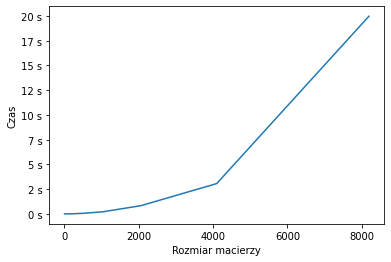
\includegraphics[width=15cm]{inverse_time.png}
  \caption{Wykres czasu od rozmiaru macierzy.}
\end{figure}

\begin{figure}[H]
  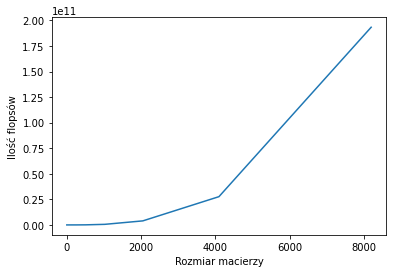
\includegraphics[width=15cm]{inverse_flops.png}
  \caption{Wykres libczby operacji od rozmiaru macierzy.}
\end{figure}
\end{center}

\subsection{Złożoność obliczeniowa}
\qquad Złożoność obliczeniowa algorytmu zależy od algorytmu mnożenia macierzy jaki został wykorzytany do obliczeń. W naszym przypadku był to algorytm Strassen'a, którego złożoność obliczeniowa wynosi: $O(n^{2.807}$).
\subsection{Porównanie rozwiązania}

Wyniki naszego algorytmu: \\
\begin{lstlisting}
%% INPUT
A = np.array([[1, 8, 5], [2, 4, 6], [3, 5, 7]])
print(recursive_matrix_inverse(A, counter))

%% OUTPUT

[[-0.1  -1.55  1.4 ]
 [ 0.2  -0.4   0.2 ]
 [-0.1   0.95 -0.6 ]]
\end{lstlisting} 
\newline
Wyniki uzyskane w numpy'u: \\

\begin{lstlisting}
%% INPUT
A = np.array([[1, 8, 5], [2, 4, 6], [3, 5, 7]])
print(np.linalg.inv(A))

%% OUTPUT

[[-0.1  -1.55  1.4 ]
 [ 0.2  -0.4   0.2 ]
 [-0.1   0.95 -0.6 ]]
\end{lstlisting}

\section{Rekurencyjna faktoryzacja LU}

\subsection{Opis algorytmu}
\qquad Algorytm dzieli macierz na 4 podmacierze, a następnie przy ich użyciu wykonuje poniższe operacje.

\begin{equation}
A = 
     \begin{pmatrix}
      A_{1,1} & A_{1,2}  \\
      A_{2,1} & A_{2,2} \\
     \end{pmatrix}
\end{equation}\\
\begin{equation}
[L_{1,1}, U_{1,1}] = LU(A_{1,1})
\end{equation}\\
\begin{equation}
[L_s, U_s]
= LU(A_{2,2} - A_{2,1}U_{1,1}^{-1}L_{1,1}^{-1}A_{1,2})
\end{equation}\\
\begin{equation}
L = 
    \begin{pmatrix}
        L_{1,1} & 0  \\         A_{2,1}U_{1,1}^{-1} & L_s \\
    \end{pmatrix}
\end{equation}\\
\begin{equation}
U = 
    \begin{pmatrix}
        U_{1,1} &  L_{1,1}^{-1}A_{1,2} \\         0 & U_s \\
    \end{pmatrix}
\end{equation}
\subsection{Pseudo-kod}
\begin{lstlisting}
def LU(A):
    if A.size > 1:
        split_at = A.shape[0] // 2
        A11, A12, A21, A22 = split(A, split_at)

        L11, U11 = LU(A11)
        U11_inv = inverse(U11)

        L21 = A21 *U11_inv
        L11_inv = inverse(L11)

        U12 = L11_inv * A12
        L22 = A22 + -A21 * U11_inv * L11_inv * A12

        Ls, Us = LU(L22)
        U22 = Us
        L22 = Ls

        return(
            [[L11, 0]
            [L21, L22]],
            
            [[U11, U12]
            [0, U22]]
            )
    else:
        return (1, A[0, 0])
\end{lstlisting}
\subsection{Benchmarki}

\begin{center}
\begin{figure}[H]
  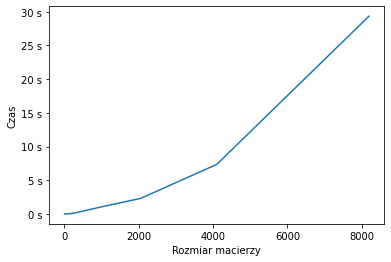
\includegraphics[width=15cm]{lu_time.png}
  \caption{Wykres czasu od rozmiaru macierzy.}
\end{figure}

\begin{figure}[H]
  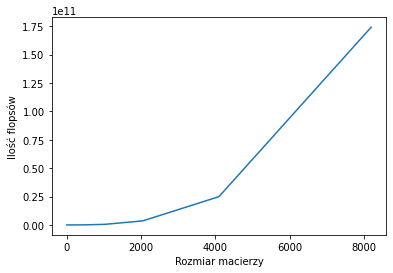
\includegraphics[width=15cm]{lu_flops.png}
  \caption{Wykres libczby operacji od rozmiaru macierzy.}
\end{figure}
\end{center}

\subsection{Złożoność obliczeniowa}

\qquad Złożoność obliczeniowa faktoryzacji LU to w przybliżeniu $O(n^{2.529})$.

\subsection{Porównanie rozwiązania}
\begin{lstlisting}
Wyniki uzyskane przez nasze implementacje:
%% INPUT
A = np.array([[1, 8, 5], [2, 4, 6], [3, 5, 7]])
L, U = recursive_lu(A, counter)
print(L)
print(U)
%% OUTPUT
[[1.        , 0.        , 0.        ],
 [2.        , 1.        , 0.        ],
 [3.        , 1.58333333, 1.        ]]

[[  1.        ,   8.        ,   5.        ],
 [  0.        , -12.        ,  -4.        ],
 [  0.        ,   0.        ,  -1.66666667]]
\end{lstlisting} \\
Wyniki w Wolframie:
\begin{center}
  \includegraphics{image.png}
  \caption{Wynik faktoryzacji LU uzyskane przy użyciu Wolframa.}
\end{center}
\section{Rekurencyjne obliczanie wyznacznika}

\subsection{Opis algorytmu}
\qquad Algorytm wykorzystuje faktoryzacja LU do obliczenia wyznacznika macierzy. Najpierw wykonujemy faktoryzacje, a następnie bierzemy wszystkie liczby z głównej przekątniej macierzy U i L, po czym mnożymi je wszystkie ze sobą. \\

\begin{equation}
[ L_{n,n}, U_{n,n} ] = LU(A_{n,n})
\end{equation}\\
\begin{equation}
U_{n,n} = 
 \begin{pmatrix}
  u_{1,1} & u_{1,2} & \cdots & u_{1,n} \\
  0 & u_{2,2} & \cdots & u_{2,n} \\
  \vdots  & \vdots  & \ddots & \vdots  \\
  0 & 0 & \cdots & u_{n,n} 
 \end{pmatrix}
\end{equation}\\
\begin{equation}
L_{n,n} = 
 \begin{pmatrix}
  1 & 0 & \cdots & 0 \\
  l_{2,1} & 1 & \cdots & 0 \\
  \vdots  & \vdots  & \ddots & \vdots  \\
  l_{n,1}  & l_{n,2}  & \cdots & 1 
 \end{pmatrix}
\end{equation}\\
\begin{equation}
det(A) = \prod_{i = 0}^{n} u_{i, i} * l_{i, i}
\end{equation}

\subsection{Pseudo-kod}
\begin{lstlisting}
def determinant(A):
    L, U = LU(A)

    U_diag = diagonal(U)

    det = 1
    for u in U_diag:
        det *= u
        
    return det
\end{lstlisting}

\subsection{Benchmarki}
\begin{center}
\begin{figure}[H]
  \includegraphics[width=15cm]{tru_time.png}
  \caption{Wykres czasu od rozmiaru macierzy.}
\end{figure}

\begin{figure}[H]
  \includegraphics[width=15cm]{tru_flops.png}
  \caption{Wykres libczby operacji od rozmiaru macierzy.}
\end{figure}
\end{center}
\subsection{Złożoność obliczeniowa}

\qquad Złożoność obliczeniowa algorytmu zależy od funkcji wyznaczającej LU oraz od rozmiaru macierzy. Wiemy także, że złożoność obliczeniowa funkcji faktoryzującej jest zależna od rozmiaru macierzy i nie jest ona liniowa. Ostatecznie więc uzyskujemy: $O(n^{2.529})$

\subsection{Porównanie rozwiązania}
Wyniki naszego algorytmu: \\
\begin{lstlisting}
%% INPUT
A = np.array([[1, 8, 5], [2, 4, 6], [3, 5, 7]])
print(recursive_determinant(A, counter))

%% OUTPUT

20.000000000000004
\end{lstlisting} 
Wyniki uzyskane w numpy'u: \\

\begin{lstlisting}
%% INPUT
A = np.array([[1, 8, 5], [2, 4, 6], [3, 5, 7]])
print(np.linalg.det(A))

%% OUTPUT

19.999999999999996
\end{lstlisting}
Natomiast według Wolframa wyznacznik wynosi równe 20.
\end{document}
